% Section content template for individual Educative lessons
% This file contains the actual content for a specific section
% Generated from Educative API section content

% Section: System Design: The Rate Limiter
% Section ID: 4770834422169600
% Section Slug: system-design-the-rate-limiter
% Generated: 2025-12-07T21:28:52.308323

\subsection{What is a rate limiter?}\label{wIGBzP2PBWxJLW-ApTT9C}
\\
A \textbf{rate limiter}, as the name suggests, puts a limit on the number of requests a service fulfills. It throttles requests that cross the predefined limit. For example, a client using a particular service's API that is configured to allow 500 requests per minute would block further incoming requests for the client if the number of requests the client makes exceeds that limit.

\begin{figure}[htbp]
 \centering
 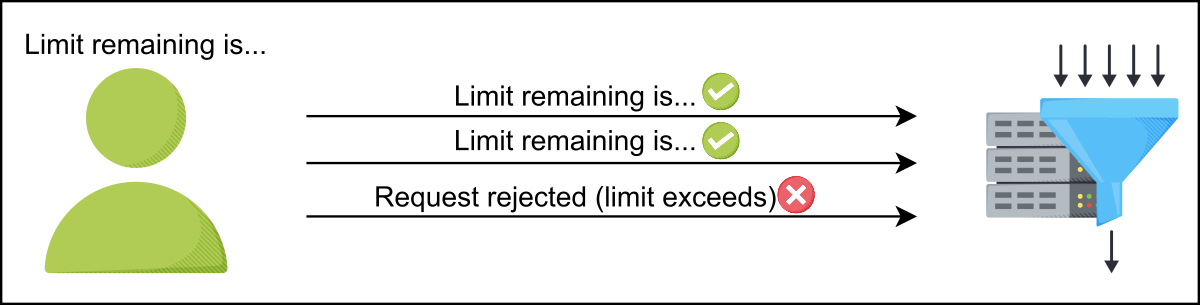
\includegraphics[width=0.5\textwidth]{Images/chapter_19/section_4770834422169600/5378385448927232.png}
 
\end{figure}

\subsection{Why do we need a rate limiter?}\label{k56alVibbC8-6y_FWFquz}
\\
A rate limiter is generally used as a defensive layer for services to avoid their excessive usage, whether intended or unintended. It also protects services against abusive behaviors that target the application layer, such as denial-of-service (DOS)DOS attacks and brute-force password attempts.
\\
Below, we have a list of scenarios where rate limiters can be used to make the service more reliable.

\begin{itemize}
\item
\protect\phantomsection\label{Gw66qwwfVQc1b9qVgAGtm}
\textbf{Preventing resource starvation:} Some denial of service incidents are caused by errors in software or configurations in the system, which causes resource starvation. Such attacks are referred to as friendly-fire denial of service. One of the common use cases of rate limiters is to avoid resource starvation caused by such denial of service attacks, whether intentional or unintentional.
\item
\protect\phantomsection\label{M6Nid1_ZsOwzQOb16eiij}
\textbf{Managing policies and quotas:} There is also a need for rate limiters to provide a fair and reasonable use of resources' capacity when they are shared among many users. The policy refers to applying limits on the time duration or quantity allocated (quota).
\item
\protect\phantomsection\label{LoV8aQ6bT-3a3afXV9icF}
\textbf{Controlling data flow:} Rate limiters could also be used in systems where there is a need to process a large amount of data. Rate limiters control the flow of data to distribute the work evenly among different machines, avoiding the burden on a single machine.
\item
\protect\phantomsection\label{6gM24ScRomU3pVuYFzwcb}
\textbf{Avoiding excess costs:} Rate limiting can also be used to control the cost of operations. For example, organizations can use rate limiting to prevent experiments from running out of control and avoid large bills. Some cloud service providers also use this concept by providing freemium services to certain limits, which can be increased on request by charging from users.
\end{itemize}

\begin{figure}[htbp]
 \centering
 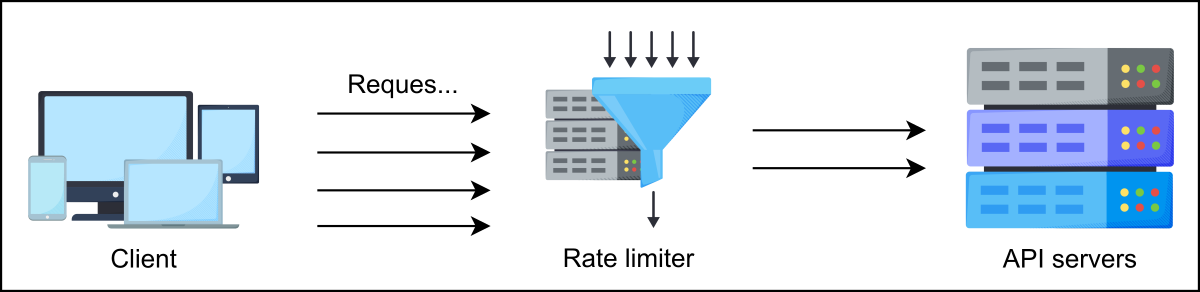
\includegraphics[width=0.5\textwidth]{Images/chapter_19/section_4770834422169600/6238621898506240.png}
 \caption{Throttling the number of requests to API servers via a rate limiter}
\end{figure}

\subsection{How will we design a rate limiter?}\label{Wiksk3s5o8xaWaXX0OhP7}
\\
In the following lessons, we will learn about the following:

\begin{enumerate}
\item
\protect\phantomsection\label{h3K4yR6eE8shEZqgr3Ck9}
\href{https://www.educative.io/courses/grokking-the-system-design-interview/requirements-of-a-rate-limiters-design}{\textbf{Requirements:}} This is where we discuss the functional and non-functional requirements of the rate limiter. We also describe the types of throttling and locations where a rate limiter can be placed to perform its functions efficiently.
\item
\protect\phantomsection\label{WpK_1_9HwDyBDgUbz-9mi}
\href{https://www.educative.io/courses/grokking-the-system-design-interview/design-of-a-rate-limiter}{\textbf{High-level design:}} In this section, we look at the high-level design to provide an overview of a rate limiter.
\item
\protect\phantomsection\label{0Pg3Zqcu9W4IGfKvKDBLc}
\href{https://www.educative.io/courses/grokking-the-system-design-interview/design-of-a-rate-limiter\#Detailed-design}{\textbf{Detailed design:}} In this section, we discuss the detailed design of a rate limiter and explain various building blocks involved in the detailed design.
\item
\protect\phantomsection\label{h8uuI1SAnB5HdFOQf2xCm}
\href{https://www.educative.io/courses/grokking-the-system-design-interview/rate-limiter-algorithms}{\textbf{Rate limiter algorithms:}} In this lesson, we explain different algorithms that play a vital role in the operations of a rate limiter.
\item
\protect\phantomsection\label{exFvNzQltEkiIFKlUS0Uw}
\href{https://www.educative.io/courses/grokking-the-system-design-interview/quiz-on-the-rate-limiters-design}{\textbf{Quiz}}\textbf{:} To assess your understanding of rate limiters, we've provided a quiz at the end of this chapter.
\end{enumerate}
\\
In the next lesson, let's start by understanding the requirements and design of a rate limiter.

% End of section content